% Practice Test 12 — Texas Edition
% Questions: 30 (17 MC + 13 SA)
% Generated by scripts/generate_practice_tests.py

\begin{practiceQuestion}{1-3-q20}{sa}
\begin{questionText}
A store sells ribbon at a constant price per yard. If $3$ yards cost $\$4.50$, what is the constant of proportionality?
\end{questionText}
\correctAnswer{$k = \$1.50$ per yard}
\explanation{$k = \frac{4.50}{3} = 1.50$ dollars per yard.}
\end{practiceQuestion}

\begin{practiceQuestion}{1-6-q20}{sa}
\begin{questionText}
A cyclist rides $42$ miles in $3$ hours. At this rate, how long does it take to ride $98$ miles?
\end{questionText}
\correctAnswer{$7$ hours}
\explanation{Rate: $42 \div 3 = 14$ mph. Time: $98 \div 14 = 7$ hours.}
\end{practiceQuestion}

\begin{practiceQuestion}{2-1-q19}{sa}
\begin{questionText}
What is $65\%$ of $140$?
\end{questionText}
\correctAnswer{$91$}
\explanation{$65\% = 0.65$. Multiply: $0.65 \times 140 = 91$.}
\end{practiceQuestion}

\begin{practiceQuestion}{2-3-q21}{sa}
\begin{questionText}
What multiplier represents a $5\%$ increase?
\end{questionText}
\correctAnswer{$1.05$}
\explanation{$1 + 0.05 = 1.05$.}
\end{practiceQuestion}

\begin{practiceQuestion}{2-6-q10}{mc}
\begin{questionText}
A student borrows $\$4{,}000$ at $7\%$ simple interest for $5$ years. What is the total amount owed?
\end{questionText}
\choiceA{$\$1{,}400$}
\choiceB{$\$4{,}700$}
\choiceC{$\$5{,}400$}
\choiceD{$\$5{,}600$}
\correctAnswer{C}
\explanation{$I = 4{,}000 \times 0.07 \times 5 = \$1{,}400$. Total $= 4{,}000 + 1{,}400 = \$5{,}400$.}
\end{practiceQuestion}

\begin{practiceQuestion}{2-8-q29}{gsa}
\begin{questionText}
The table shows two credit card offers. You plan to charge $\$600$ and pay it back after $1$ year. How much less does Card A cost you in total?

\begin{center}
\begin{tabular}{|l|c|c|}
\hline
 & \textbf{Card A} & \textbf{Card B} \\
\hline
Annual Interest Rate & $10\%$ & $22\%$ \\
\hline
Annual Fee & $\$25$ & $\$0$ \\
\hline
\end{tabular}
\end{center}
\end{questionText}
\correctAnswer{$\$47$}
\explanation{Card A: interest $= 600 \times 0.10 = \$60$, plus $\$25$ fee $= \$85$ extra. Card B: interest $= 600 \times 0.22 = \$132$. Difference: $132 - 85 = \$47$. Card A saves $\$47$.}
\end{practiceQuestion}

\begin{practiceQuestion}{2-9-q23}{sa}
\begin{questionText}
A savings account earns $4\%$ per year. You deposit $\$750$ for $1$ year. How much interest do you earn?
\end{questionText}
\correctAnswer{$\$30$}
\explanation{$I = 750 \times 0.04 = \$30$.}
\end{practiceQuestion}

\begin{practiceQuestion}{2-10-q27}{gmc}
\begin{questionText}
The line graph below shows two accounts over $3$ years, both starting at $\$500$ with $10\%$ interest. Which line represents compound interest?

\begin{center}
\begin{tikzpicture}[scale=0.8]
  \draw[thick,->] (0,0) -- (5,0) node[right] {Year};
  \draw[thick,->] (0,0) -- (0,5) node[above] {\$};
  \foreach \x in {0,1,2,3} {
    \draw (\x+0.5,-0.1) -- (\x+0.5,0.1);
    \node[below] at (\x+0.5,-0.15) {\footnotesize \x};
  }
  \foreach \y/\label in {1/500, 2/550, 3/600, 4/650} {
    \draw (-0.1,\y) -- (0.1,\y);
    \node[left] at (-0.15,\y) {\footnotesize \$\label};
  }
  % Simple (Line A) - straight line
  \draw[thick,funRed,mark=square*] plot coordinates {(0.5,1) (1.5,2) (2.5,3) (3.5,4)};
  \node[right,funRed] at (3.7,4) {\footnotesize Line A};
  % Compound (Line B) - curved
  \draw[thick,funBlue,mark=*] plot coordinates {(0.5,1) (1.5,2.1) (2.5,3.32) (3.5,4.65)};
  \node[right,funBlue] at (3.7,4.65) {\footnotesize Line B};
\end{tikzpicture}
\end{center}
\end{questionText}
\choiceA{Line A}
\choiceB{Line B}
\choiceC{Both lines}
\choiceD{Neither line}
\correctAnswer{B}
\explanation{Compound interest grows by increasing amounts each year, so the curve bends upward. Line B is compound; Line A (straight) is simple.}
\end{practiceQuestion}

\begin{practiceQuestion}{4-1-q20}{sa}
\begin{questionText}
Evaluate $-3x + 14$ when $x = -5$.
\end{questionText}
\correctAnswer{$29$}
\explanation{Substitute: $-3(-5) + 14 = 15 + 14 = 29$.}
\end{practiceQuestion}

\begin{practiceQuestion}{4-2-q10}{mc}
\begin{questionText}
Simplify $2.5a + 1.3 - 0.5a + 2.7$.
\end{questionText}
\choiceA{$2a + 4$}
\choiceB{$3a + 4$}
\choiceC{$2a - 4$}
\choiceD{$6$}
\correctAnswer{A}
\explanation{Combine variable terms: $2.5a - 0.5a = 2a$. Combine constants: $1.3 + 2.7 = 4$. Result: $2a + 4$.}
\end{practiceQuestion}

\begin{practiceQuestion}{5-3-q24}{sa}
\begin{questionText}
Solve $-8(x + 2) = 24$.
\end{questionText}
\correctAnswer{$x = -5$}
\explanation{Divide by $-8$: $x + 2 = -3$. Subtract $2$: $x = -5$. Check: $-8(-5 + 2) = -8(-3) = 24$ \checkmark.}
\end{practiceQuestion}

\begin{practiceQuestion}{5-4-q15}{mc}
\begin{questionText}
Solve $\dfrac{5x}{2} + 3 = 18$.
\end{questionText}
\choiceA{$x = 3$}
\choiceB{$x = 6$}
\choiceC{$x = 42$}
\choiceD{$x = 15$}
\correctAnswer{B}
\explanation{Subtract $3$: $\frac{5x}{2} = 15$. Multiply by $2$: $5x = 30$. Divide by $5$: $x = 6$. Check: $\frac{5(6)}{2} + 3 = 15 + 3 = 18$ \checkmark.}
\end{practiceQuestion}

\begin{practiceQuestion}{5-5-q03}{mc}
\begin{questionText}
Which inequality represents ``at most $15$''?
\end{questionText}
\choiceA{$x > 15$}
\choiceB{$x < 15$}
\choiceC{$x \geq 15$}
\choiceD{$x \leq 15$}
\correctAnswer{D}
\explanation{``At most'' means $15$ or less, which is $x \leq 15$.}
\end{practiceQuestion}

\begin{practiceQuestion}{5-6-q16}{mc}
\begin{questionText}
Solve $\dfrac{x}{2} - 3 > 1$ and describe the graph.
\end{questionText}
\choiceA{Open circle at $8$, shade right}
\choiceB{Closed circle at $8$, shade right}
\choiceC{Open circle at $4$, shade right}
\choiceD{Open circle at $8$, shade left}
\correctAnswer{A}
\explanation{Add $3$: $\frac{x}{2} > 4$. Multiply by $2$: $x > 8$. Open circle at $8$, shade right.}
\end{practiceQuestion}

\begin{practiceQuestion}{6-2-q09}{mc}
\begin{questionText}
A map uses $1$ cm $= 40$ km. A lake is $3$ cm wide on this map. You redraw the map at $1$ cm $= 8$ km. How wide is the lake on the new map?
\end{questionText}
\choiceA{$0.6$ cm}
\choiceB{$5$ cm}
\choiceC{$15$ cm}
\choiceD{$24$ cm}
\correctAnswer{C}
\explanation{Scale ratio: $\frac{40}{8} = 5$. New width: $3 \times 5 = 15$ cm.}
\end{practiceQuestion}

\begin{practiceQuestion}{6-3-q27}{gmc}
\begin{questionText}
The diagram shows a triangle with the given measurements. How many different triangles can be drawn with these exact conditions?

\begin{center}
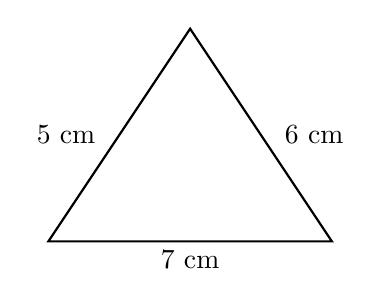
\begin{tikzpicture}[scale=0.9]
  \draw[thick] (0,0) -- (4,0) -- (2,3) -- cycle;
  \node[below] at (2,0) {$7$ cm};
  \node[left] at (0.8,1.5) {$5$ cm};
  \node[right] at (3.2,1.5) {$6$ cm};
\end{tikzpicture}
\end{center}
\end{questionText}
\choiceA{None}
\choiceB{Exactly one}
\choiceC{Exactly two}
\choiceD{Infinitely many}
\correctAnswer{B}
\explanation{Three side lengths that satisfy the triangle inequality (SSS) produce exactly one unique triangle. Check: $5 + 6 = 11 > 7$, $5 + 7 = 12 > 6$, $6 + 7 = 13 > 5$. All pass.}
\end{practiceQuestion}

\begin{practiceQuestion}{6-4-q15}{mc}
\begin{questionText}
You know two angles of a triangle are $55°$ and $65°$ and a non-included side is $9$ cm. This is an example of:
\end{questionText}
\choiceA{SSS}
\choiceB{SAS}
\choiceC{ASA}
\choiceD{AAS}
\correctAnswer{D}
\explanation{Two angles and a non-included side is AAS (Angle-Angle-Side). This produces a unique triangle.}
\end{practiceQuestion}

\begin{practiceQuestion}{6-5-q02}{mc}
\begin{questionText}
You slice a cylinder with a horizontal cut parallel to its base. What shape is the cross-section?
\end{questionText}
\choiceA{Rectangle}
\choiceB{Circle}
\choiceC{Oval}
\choiceD{Triangle}
\correctAnswer{B}
\explanation{A horizontal cut through a cylinder parallel to the circular base produces a circle.}
\end{practiceQuestion}

\begin{practiceQuestion}{6-8-q23}{sa}
\begin{questionText}
A scale model of a bridge is $18$ inches long. The actual bridge is $900$ feet long. What is the scale factor (as a ratio of model to actual)?
\end{questionText}
\correctAnswer{$1:600$}
\explanation{Convert $900$ ft to inches: $900 \times 12 = 10{,}800$ inches. Scale: $\frac{18}{10{,}800} = \frac{1}{600}$. The ratio is $1:600$.}
\end{practiceQuestion}

\begin{practiceQuestion}{7-4-q24}{sa}
\begin{questionText}
A shape is made of two congruent triangles, each with base $8$ cm and height $5$ cm, joined along their bases. What is the total area?
\end{questionText}
\correctAnswer{$40$ cm$^2$}
\explanation{Each triangle: $\frac{1}{2} \times 8 \times 5 = 20$ cm$^2$. Two triangles: $20 + 20 = 40$ cm$^2$.}
\end{practiceQuestion}

\begin{practiceQuestion}{7-5-q28}{gmc}
\begin{questionText}
The diagram shows a triangular prism. What is its total surface area?

\begin{center}
\begin{tikzpicture}[scale=0.4]
  % Front triangle
  \draw[thick,funBlue,fill=funBlue!10] (0,0) -- (6,0) -- (3,4) -- cycle;
  % Back triangle (offset)
  \draw[thick,funBlue,fill=funBlue!20] (2,1.5) -- (8,1.5) -- (5,5.5) -- cycle;
  % Connecting edges
  \draw[thick,funBlue] (0,0) -- (2,1.5);
  \draw[thick,funBlue] (6,0) -- (8,1.5);
  \draw[thick,funBlue] (3,4) -- (5,5.5);
  % Labels
  \node[below] at (3,0) {$6$ cm};
  \node[left] at (1.2,2) {$5$ cm};
  \node[right] at (4.8,2) {$5$ cm};
  \node[right] at (8,3.5) {$8$ cm};
  \node[above left] at (1,0.8) {$h = 4$ cm};
\end{tikzpicture}
\end{center}
\end{questionText}
\choiceA{$104$ cm$^2$}
\choiceB{$128$ cm$^2$}
\choiceC{$152$ cm$^2$}
\choiceD{$160$ cm$^2$}
\correctAnswer{C}
\explanation{Two triangles: $2 \times \frac{1}{2} \times 6 \times 4 = 24$ cm$^2$. Three rectangles: $6 \times 8 + 5 \times 8 + 5 \times 8 = 48 + 40 + 40 = 128$ cm$^2$. Total: $24 + 128 = 152$ cm$^2$.}
\end{practiceQuestion}

\begin{practiceQuestion}{7-6-q05}{mc}
\begin{questionText}
A triangular prism has a base that is a triangle with base $8$ cm and height $3$ cm. The prism is $10$ cm long. What is the volume?
\end{questionText}
\choiceA{$24$ cm$^3$}
\choiceB{$80$ cm$^3$}
\choiceC{$120$ cm$^3$}
\choiceD{$240$ cm$^3$}
\correctAnswer{C}
\explanation{$B = \frac{1}{2} \times 8 \times 3 = 12$ cm$^2$. $V = Bh = 12 \times 10 = 120$ cm$^3$.}
\end{practiceQuestion}

\begin{practiceQuestion}{8-1-q30}{gsa}
\begin{questionText}
The table shows the results of a random sample of $80$ people about their preferred pet.

\begin{center}
\begin{tabular}{|l|c|}
\hline
\textbf{Pet} & \textbf{Number} \\
\hline
Dog & $32$ \\
\hline
Cat & $24$ \\
\hline
Fish & $12$ \\
\hline
Bird & $8$ \\
\hline
Other & $4$ \\
\hline
\end{tabular}
\end{center}

What percent of the sample prefers cats? If the population is $5{,}000$, predict how many prefer cats.
\end{questionText}
\correctAnswer{$30\%$; $1{,}500$ people}
\explanation{$\frac{24}{80} = 0.30 = 30\%$. Then $30\%$ of $5{,}000 = 1{,}500$.}
\end{practiceQuestion}

\begin{practiceQuestion}{8-2-q17}{mc}
\begin{questionText}
A dentist's office randomly surveys $30$ patients and finds that the mean number of cavities is $1.5$. The office has $900$ patients. Predict the total number of cavities among all patients.
\end{questionText}
\choiceA{$450$}
\choiceB{$900$}
\choiceC{$1{,}350$}
\choiceD{$1{,}500$}
\correctAnswer{C}
\explanation{$900 \times 1.5 = 1{,}350$ total cavities.}
\end{practiceQuestion}

\begin{practiceQuestion}{8-4-q07}{mc}
\begin{questionText}
Data set: $5, 8, 10, 12, 15, 18, 50$. Which measure of variability is most affected by the outlier $50$?
\end{questionText}
\choiceA{IQR}
\choiceB{Median}
\choiceC{Range}
\choiceD{Mode}
\correctAnswer{C}
\explanation{Range $= 50 - 5 = 45$, which is heavily influenced by the outlier. IQR ignores the extremes and is less affected.}
\end{practiceQuestion}

\begin{practiceQuestion}{8-5-q03}{mc}
\begin{questionText}
A stem-and-leaf plot has the row: $3 \mid 1\;4\;4\;7\;9$. How many data values are in this row?
\end{questionText}
\choiceA{$3$}
\choiceB{$4$}
\choiceC{$5$}
\choiceD{$25$}
\correctAnswer{C}
\explanation{Count the leaves: $1, 4, 4, 7, 9$ — that's $5$ data values ($31, 34, 34, 37, 39$).}
\end{practiceQuestion}

\begin{practiceQuestion}{8-6-q21}{sa}
\begin{questionText}
A circle graph shows a budget of $\$2{,}000$. The housing sector is $40\%$. How much is spent on housing?
\end{questionText}
\correctAnswer{$\$800$}
\explanation{$40\%$ of $\$2{,}000 = 0.40 \times 2{,}000 = \$800$.}
\end{practiceQuestion}

\begin{practiceQuestion}{9-4-q15}{mc}
\begin{questionText}
Which of these is NOT a valid probability model?
\end{questionText}
\choiceA{$P(A) = 0.5$, $P(B) = 0.5$}
\choiceB{$P(A) = 0.7$, $P(B) = 0.2$, $P(C) = 0.1$}
\choiceC{$P(A) = 0.6$, $P(B) = 0.6$}
\choiceD{$P(A) = 1$}
\correctAnswer{C}
\explanation{$0.6 + 0.6 = 1.2 > 1$. The probabilities must sum to exactly $1$.}
\end{practiceQuestion}

\begin{practiceQuestion}{9-6-q25}{sa}
\begin{questionText}
Three coins are flipped. What is the probability of getting exactly $1$ head? Write your answer as a fraction in simplest form.
\end{questionText}
\correctAnswer{$\frac{3}{8}$}
\explanation{Outcomes with exactly $1$ head: HTT, THT, TTH — that is $3$ out of $8$. $P = \frac{3}{8}$.}
\end{practiceQuestion}

\begin{practiceQuestion}{9-7-q14}{mc}
\begin{questionText}
Mia uses a random number generator to produce digits $0$--$9$. She runs $20$ trials to simulate a $40\%$ chance of an event. In her simulation, the event happens $10$ times. What is the experimental probability?
\end{questionText}
\choiceA{$0.20$}
\choiceB{$0.40$}
\choiceC{$0.50$}
\choiceD{$0.10$}
\correctAnswer{C}
\explanation{$P = \frac{10}{20} = 0.50$. This is higher than the theoretical $0.40$, but with only $20$ trials, variation is expected.}
\end{practiceQuestion}
